%analysis and design
\iffalse
Analysis and Design
high level overview of the design - differences to previous design
if not fully implemented - explain why
description of design in retrospect - doesnt need to be in order
where reasoned changes in design occured, inlcude these
Make sure to identify points where key design decisions were made, what were other options, why
make example of tradeoffs
\fi

\chapter{Analysis \& Design}
The central aim of this project was to be produce a HLS framework to transform Julia code into HDL, and structure the toolchain so that it can be expanded upon in future work. As such, the priority was creating a structural flow that took a subset of Julia source code and transformed it into HDL that is synthesisable and can be tested in simulation. This is contained inside two Julia packages: SSATools and Dynamic Scheduling. These deviated from the original planned flow by reducing the subset of the language covered and altering the scheduling methods. The components of the final design and the deviations from the original flow shall be outlined in the following chapter.

\section{Flow Overview}
%julia sourcecode - IR transform - CDFG info extraction - dynamic shceduling - vhdl conversion
\begin{figure}[htb!]
    \centering
    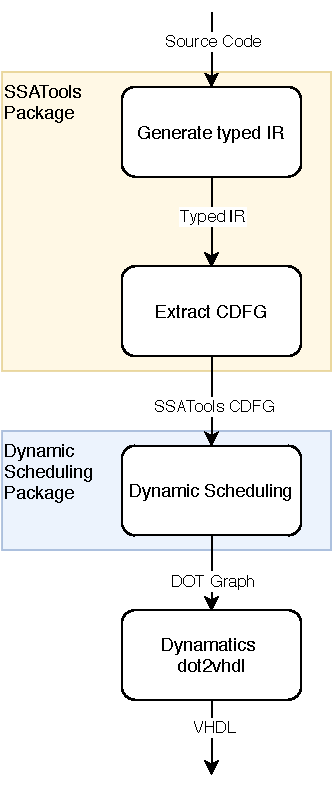
\includegraphics[width=0.3\textwidth]{Images/basic_flow.pdf}
    \caption{Overview of the main stages in the Julia HLS flow.}
    \label{fig:julia_flow_overview}
\end{figure}

The flow consists of the four main stages shown in Figure \ref{fig:julia_flow_overview}, beginning with the generation of the typed IR from the source code. The function source code is passed into the SSATools package along with the type information for the arguments of the function. This allows the tool to use the standard reflection method \code{@code\_typed} to generate the typed IR. The typed IR contains a large amount of useful information to be extracted and presented in the SSATools CDFG type. The benefits of the CDFG type include the separation of argument information and operation information in different array. This simplifies the generation of the argument components (\code{entry}) as their information is now condensed into array entries to be iterated over in the same way as the operations.

The Dynamic Scheduling package takes inspiration from the dynamatic library \cite{dyn_lib} with the key differences being the input type, intermediary representation of the elastic circuit type and the language used to perform the CDFG passes necessary to generate digital hardware. The benefits of modelling the Dynamic Scheduling package on the existing Dynamatic library are that the Julia flow can make use of the generic VHDL components in the library as well as the dot2vhdl parser to convert the resulting DOT graph output to a VHDL file. 

The flow was designed in this fashion to be modular. The CDFG produced at the output of the SSATools package will be the standard interface for the existing Dynamic Scheduling package as well as future allocation, binding and static scheduling packages.

\section{Design Choices}

\subsection{Julia Typed IR} %TODO where existing flows mentioned, add refs
Existing HLS flows using the C/C++ language make use LLVM IR as the starting point for the conversion. The main benefit of using the LLVM IR compared to the raw C code is that source code is formalised and structured by the compiler into a series of operations that are machine independent. These operations are sequential and chained together within basic blocks that provide an explicit control flow that would not be obvious when parsing source code. The key disadvantage of using Julia's LLVM IR is the significant increase in operations and control information required for a typical program. This stems from Julia's capability to use dynamically typed code, which results in the compiler automatically adding additional operations for error correction and memory management. These operations are added in at the higher-level representations of the code as single line statements to be expanded at the LLVM layer. The same expansion can apply to some of the Base Julia operations used in the typed IR. 

The typed IR has the benefits of the LLVM IR in that it has a similar well structured SSA form from which branching and looping control structures can be determined.  The typed IR is high-level enough that additional error and memory management operations have not been expanded and can be altered or removed more easily. The typed IR is also low-level enough that the majority of the complex functions have been deconstructed into simpler Base operations which can be mapped to the fundamental functional operations with hardware equivalents. These reasons are the primary motivation behind choosing to use the Julia typed IR as the HLS formal representation over the LLVM IR.

\subsection{SSATools Package}
A disadvantage of using the Julia typed IR was the lack of existing tools and documentation compared to LLVM. This motivated the creation of the SSATools package. The primary goal of this package is to parse the source code and extract the control and data flow information used by the rest of the HLS flow. The tool makes use of the existing Julia reflection methods to generate the typed IR, and then iterates through each line of the IR to create a \code{CDFGNode} for each of the operations. For each operation, the input values are recorded in the node, along with their datatype, position in the operation, and whether or not they are constants, SSA values or the program arguments. This preserves the data dependencies in the predecessor direction. Iterating over the new \code{CDFGNodes} is then done to construct the data dependencies in the successor direction.

The secondary aim of the SSATools package is to implement IR and CDFG passes that can be used to optimise the CDFG for the scheduling process. In the current form of the package, the additional methods can be used to make alterations by inserting and deleting lines in the typed IR. A set of conversion methods was also added to the package to verify changes to the IR would not affect the correctness of the function. These methods allow for the verification of the typed IR alterations by transforming the new typed IR into an anonymous function where the output can be compared to the expected output from the original function. This forms the starting point for IR passes to be implemented in future work. 

The majority of Julia functions rely completely on Julia Base operations in the typed IR, however some functions can use functions that are outside of the base Julia library and are dynamically called into. The current form of the SSATools package does not support these called non-Base methods as many cannot be automatically converted to an FPGA equivalent. In preparation for future work to support these operations, a method to decompose a non-Base function into its equivalent Base functions was added. 

\subsection{Scheduling}
Figure \ref{fig:static_simple} demonstrates the basic sections of a statically scheduled piece of hardware. The Finite State Machine (FSM) controller is responsible for dictating the entire program flow, and is determined from the CDFG prior to execution and remains unchanged throughout the program. Figure \ref{fig:dynamic_simple} is an example of a dynamically scheduled hardware. The hardware operations are wrapped in a communication layer that inherently determines the control flow. This means that the connections within the CDFG can be explicitly mapped to hardware and reduces the computation required to calculate a predetermined control flow. 

The initial plan was to use static scheduling methods to create the schedule for the HLS flow. Existing scheduling algorithms proved time consuming to implement, and would not be guaranteed to function as expected with the SSATools package output in it's previous form. We chose to switch the implementation from static scheduling to dynamic scheduling to combine the allocation and scheduling aspects of the HLS flow and reduce the complexity of producing hardware.

The main disadvantages of dynamic scheduling is the increased resource usage and increased latency. There is a significant resource overhead in adding the communication wrappers and mapping the control flow into additional components to support constructs like branches. The dynamically scheduled operations are combined in chains, reducing the maximum frequency at which the circuit can function, and therefore increasing latency. The trade off in area and latency for reduced complexity was necessary to construct enough sections of the flow to produce hardware.

\begin{figure}[htb!]
    \centering
    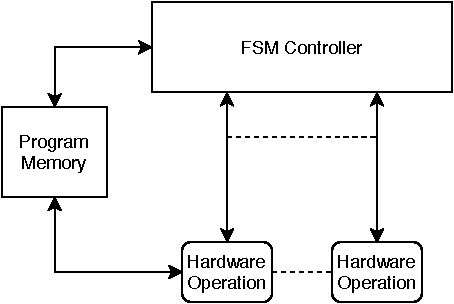
\includegraphics[width=0.5\textwidth]{Images/oversimplified_static.pdf}
    \caption{Simplified diagram of a statically scheduled program.}
    \label{fig:static_simple}
\end{figure}

\begin{figure}[htb!]
    \centering
    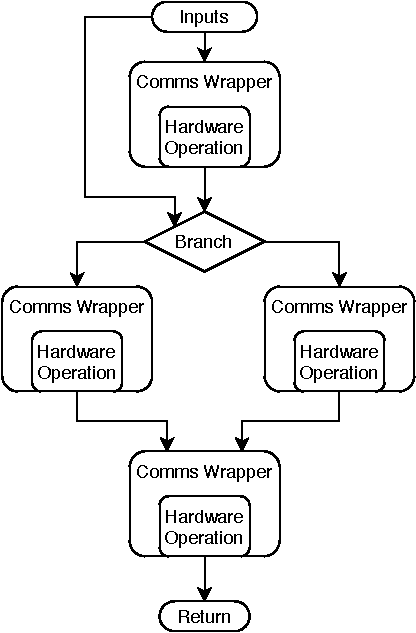
\includegraphics[width=0.5\textwidth]{Images/oversimplified_dyn.pdf}
    \caption{Simplified diagram of a dynamically scheduled program.}
    \label{fig:dynamic_simple}
\end{figure}